\documentclass{article}
\usepackage[utf8]{inputenc}
\usepackage{graphicx}
\graphicspath{ {./figure/} }
\usepackage{wrapfig}
\usepackage{listings}
\usepackage{float}
\usepackage{indentfirst}
% \graphicspath{{./}}
\title{Interfacing LCD and Ultrasonic Sensor with Arduino using Arduino-Python toolkit}
\author{Deepam Priyadarshi \thanks{Under the guidance of Dr. Subbulakshmi P, Vellore Institute of Technology, Chennai}}
\date{}

\begin{document}

\begin{center}
		\textbf{\huge FOSSEE Arduino Internship\\Vellore Institute of Technology, Chennai\\}
		\vspace{30pt}
		
\includegraphics[width=0.7\textwidth]{./logo.png} \\
		
\includegraphics[width=0.7\textwidth]{./fossee.png} \\
		\vspace{20pt}
		\textbf{\Large Interfacing LCD and Ultrasonic Sensor with Arduino using Arduino-Python toolkit\\}
		\vspace{30pt}
		\textit{By\\}
		\textbf{\large Deepam Priyadarshi\\}
		\vspace{20pt}
		\textit{Under the kind guidance of}\\
		\textbf{\large Dr. Subbulakshmi P}\\
		\vspace{35pt}
		\textit{Submitted to}\\
		\textbf{\large FOSSEE Club\\
			Vellore Institute of Technology, Chennai\\
			August 30, 2021
		}
\end{center}
\pagebreak
\maketitle

\section{Abstract}
The objective of this project is to perform the experiment of measuring the distance of an obstacle using HC-SR04 ultrasonic sensor and displaying the results onto a 16x2 character LCD. This will help students learn the LCD module of the Arduino and how to use it along with other sensors. The current FLOSS software doesn't contain any provision for interfacing the LCD module with Arduino using the existing FLOSS-Arduino python toolkit. It will make learning Arduino more easier with a programmer friendly language, Python.

\section{Preliminaries}
\subsection{LCD}
The LCD used in our experiment is a 16X2 Character LCD which has 16 columns and 2 rows for displaying unicode characters as shown in the Figure \ref{fig:16X2 Character LCD}. 
\begin{figure}[H]
    \centering
    \fbox{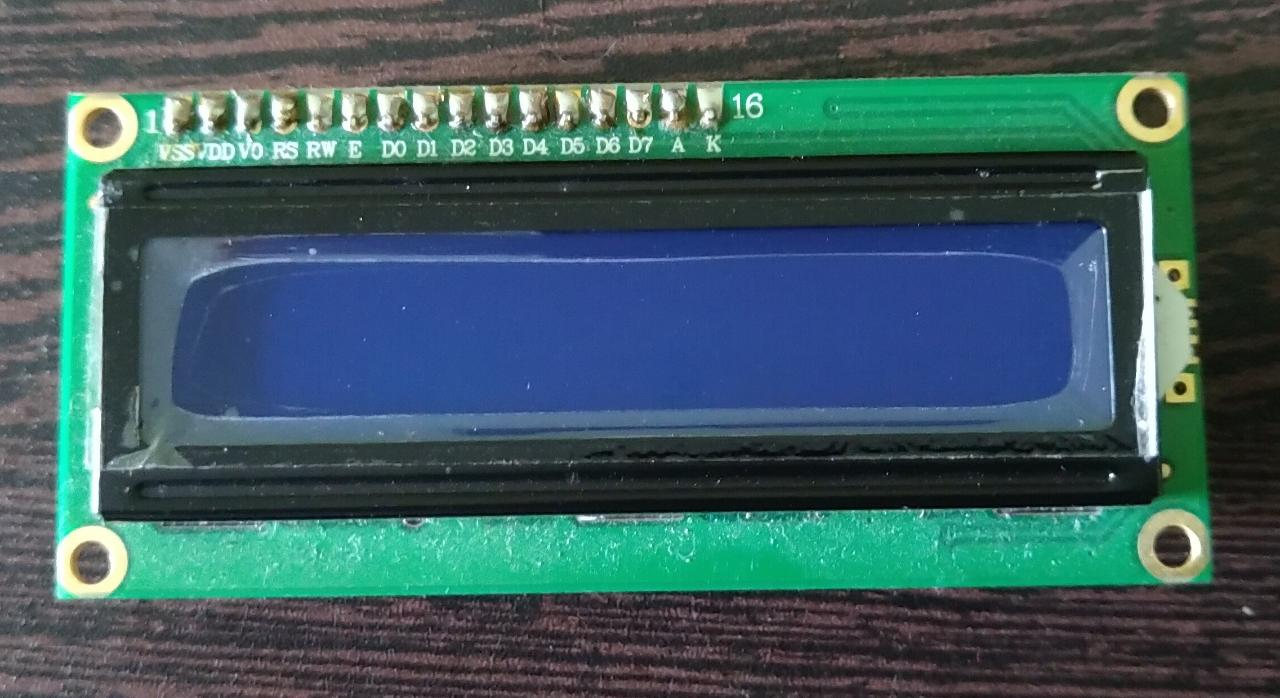
\includegraphics[width=0.5\textwidth]{LCD.jpeg}}
    \caption{16X2 Character LCD}
    \label{fig:16X2 Character LCD}
\end{figure}


Every character LCD has 16 pins as show in the Figure \ref{fig:LCD pin out} The \emph{VSS pin} is the ground supply for the LCD and the \emph{VDD pin} is the +5v power supply for the LCD. The \emph{VEE/VO pin} the LCD contrast control pin and is connected to a potentiometer to adjust the required contrast of the text display. The \emph{RS pin} is the register select pin and it differentiate between data or command that is being sent to the LCD register. A logical high on this pin enables the \emph{command mode} while a logical low on this pin enables \emph{data mode}. The \emph{RW pin} is the Read/Write pin which which toggles the read or write mode of the LCD. A logical low on this pin enables the \emph{write mode} and the data gets written to LCD, while a logical high will enable \emph{read mode} and the data is read from the LCD register. The \emph{E pin} is the enable pin which when high enables the data communication between the LCD and the microcontroller. Then their are 8 data pins \emph{D7-D0} for 8 bit data communication. At last their are two pins, \emph{LED +ve and LED -ve}, which are the power and ground supply respectively for the Backlight LED of the display.

\begin{figure}[H]
    \centering
    \fbox{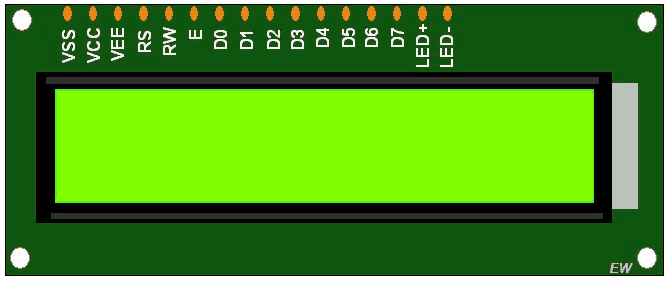
\includegraphics[width=0.5\textwidth]{PinDig.png}}
    \caption{LCD Pinouts}
    \label{fig:LCD pin out}
\end{figure}

\subsubsection{8-bit Vs. 4-bit data transfer}
In 8 bit data transfer mode all the 8 data pins of LCD are used by the microcontroller to send the 8-bit data. Since the character datatype is 8-bit wide, therefore in 8-bit mode, all the bits are sent at once. This type of communication is much faster as compared to 4-bit mode, since in this mode all the data bits are sent at once.


Whereas in 4-bit data communication mode only 4 data pins \emph{D4-D7} are used for LCD initialization. The 8-bit ASCII value is divided into two 4-bit nibbles. The higher nibbles are sent first followed by the lower nibbles. In contrast with 8-bit mode, 4-bit mode require two clock cycle for complete data transfer but it saves a lot of I/O pins of the microcontroller. 

\section{HC-SR04 Ultrasonic Sensor}
As shown in the Figure \ref{fig:ultrsonic sensor} is an Ultrasonic Sensor, HC-SR04, used for measuring the distance of an obstacle. The working principle of this sensor is based on speed of sound in air at a given temperature (\emph{for our experiment we have assumed the speed to be 340 m/s or 0.034 cm/\(\mu\)s at normal room temperature}). The sensor has the transmitter circuit on the left and the receiver circuit on the right hand side of the board. The transmitter circuit sends an ultrasound at a frequency of 40kHz which bounces back from an obstacles and is received at the receiver circuit. The time taken by the ultrasound is measured and the distance is calculated by the formula :-

\[Distance(cm) = \frac{speed * time}{2}\]
\[ = \frac{0.034 * time}{2}\]

\noindent where \emph{speed} is the speed of sound in air (0.034 cm/\(\mu\)s) and \emph{time} is the time taken by the ultrasound in \(\mu\)s.

\begin{figure}[H]
    \centering
    \fbox{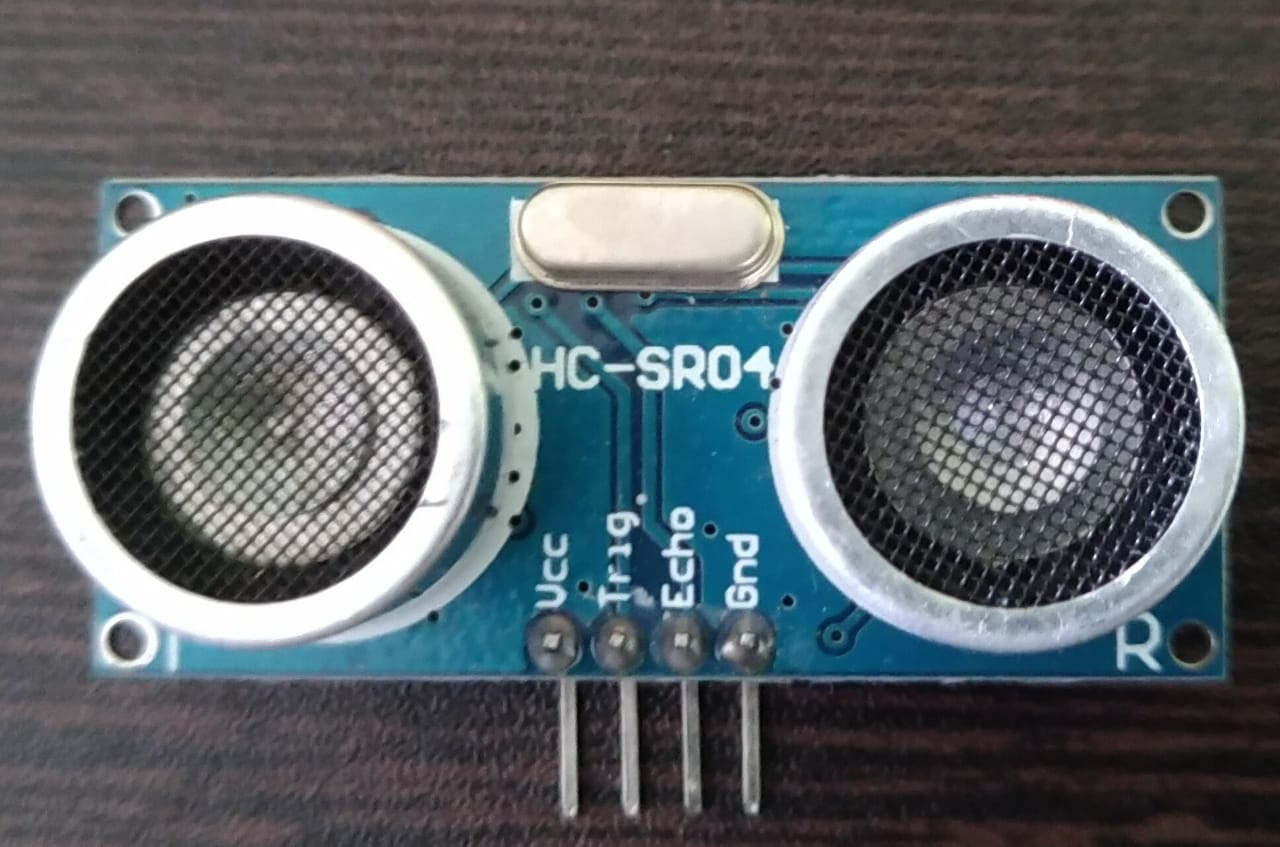
\includegraphics[width=0.5\textwidth]{Ultra.jpeg}}
    \caption{HC-SR04}
    \label{fig:ultrsonic sensor}
\end{figure}

The sensor has three pins, namely \emph{VCC, Trigger, Echo and Ground} as shown in Figure \ref{fig:ultrsonic sensor}. The \emph{VCC} and \emph{Ground} are the +5v power and Ground supply respectively for the sensor.

\begin{figure}[H]
    \centering
    \fbox{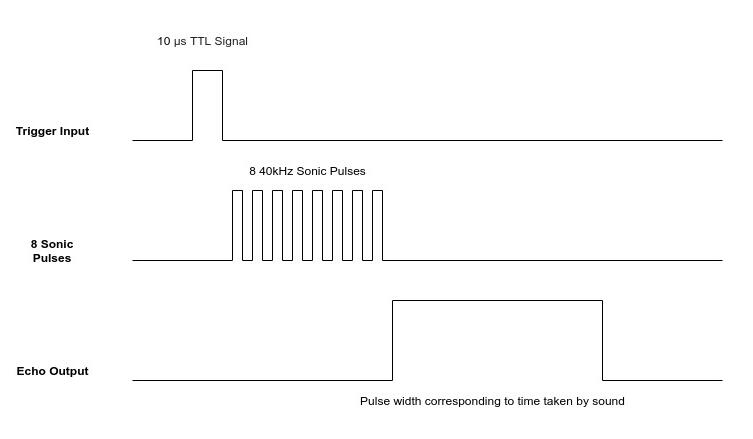
\includegraphics[width=0.8\textwidth]{TimingDig.jpeg}}
    \caption{HC-SR04 Timing Diagram}
    \label{fig:Timing Dig}
\end{figure}

The triggers pin set on logical high signal for at most 10\(\mu\)s. This will initiate the sensor to start sending sonic sounds in a 8 burst cycle at 40kHz. At the end of the 8\textsuperscript{th} sonic pulse, the echo pin is set high until the sonic pulses are received at the receiver after back from an obstacle. This duration of the high echo pulse (in \(\mu\)s) is measured by micro-controller for getting the time take by sound. A maximum of 38ms is returned if no obstacle is found. The timing diagram given in Figure \ref{fig:Timing Dig}.

\section{Connecting LCD and HC-SR04 with Arduino UNO using a breadboard}
\begin{figure}[H]
    \centering
    \fbox{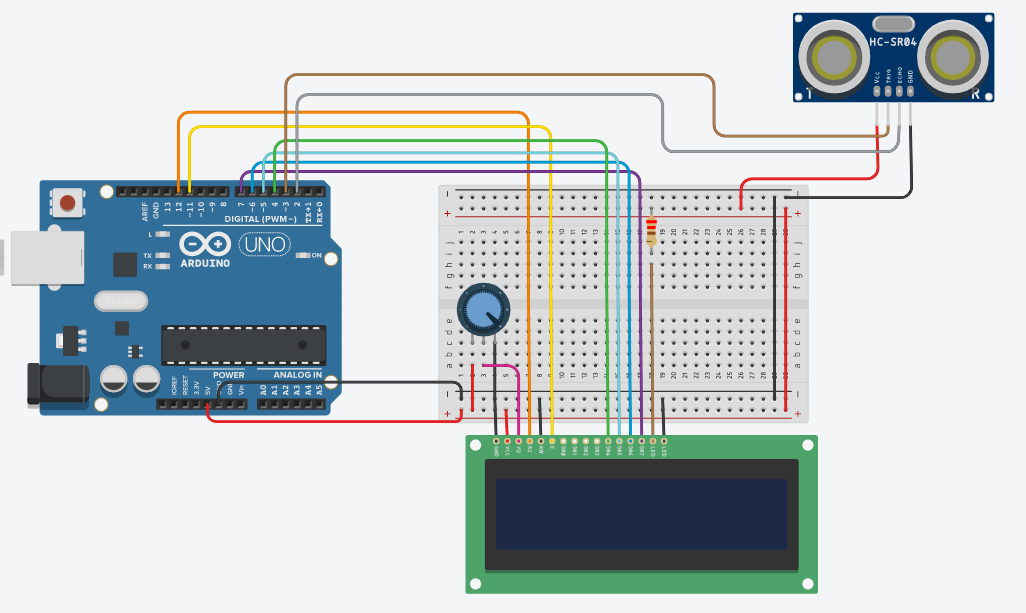
\includegraphics[width=1\textwidth]{wiring.png}}
    \caption{Wiring Connectiong}
    \label{fig:wiring}
\end{figure}
Figure \ref{fig:wiring} shows the pin connections of LCD and HC-SR04 with Arduino I/O pins. For our experiment we have used Arduino's Digital I/O pin 12, 11, 4, 5, 6 and 7 to connect with LCD's RS, VEE, D4, D5, D6 and D7 pins respectively. The \emph{VSS} and \emph{VCC} of LCD pin are connected to Arduino's ground and +5V pins respectively. And we have used pin 2 and 3 of Arduino to connect with Ultrasonic Senor's Echo and Trig pins respectively.

\section{Output Screenshots}
\subsection{For LCD interfacing}
Figure \ref{fig:lcd_run} shows the the python terminal executing the LCD the interfacing code. The code take an input of the number of columns and rows of the LCD and the text to be displayed from the user. It also ask the user whether to terminate or continue with new text to be displayed.
\begin{figure}[H]
    \centering
    \fbox{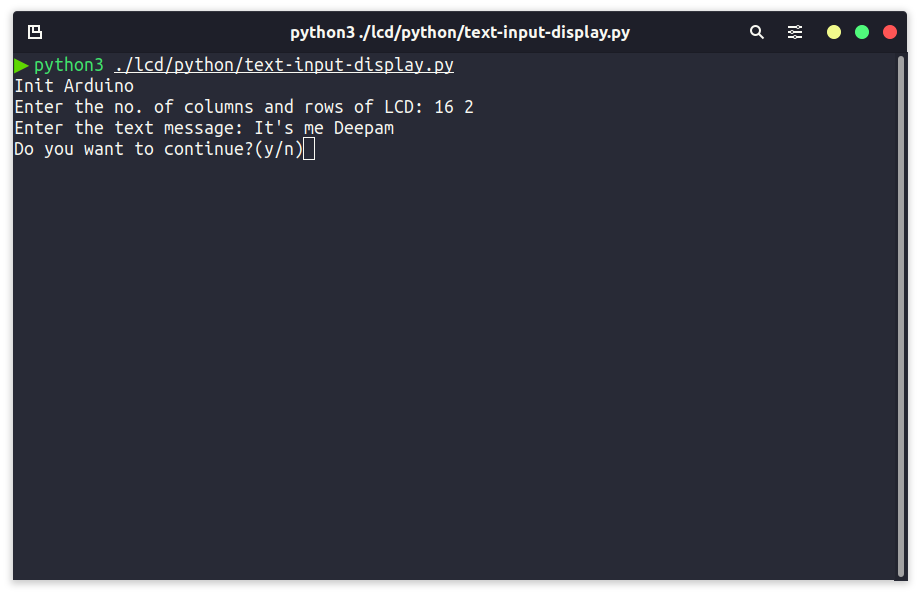
\includegraphics[width=1\textwidth]{lcd_run.png}}
    \caption{Python console executing LCD interfacin code}
    \label{fig:lcd_run}
\end{figure}


In Figure \ref{fig:lcd_output}, the LCD displays the input text received from the serial port.
\begin{figure}[H]
    \centering
    \fbox{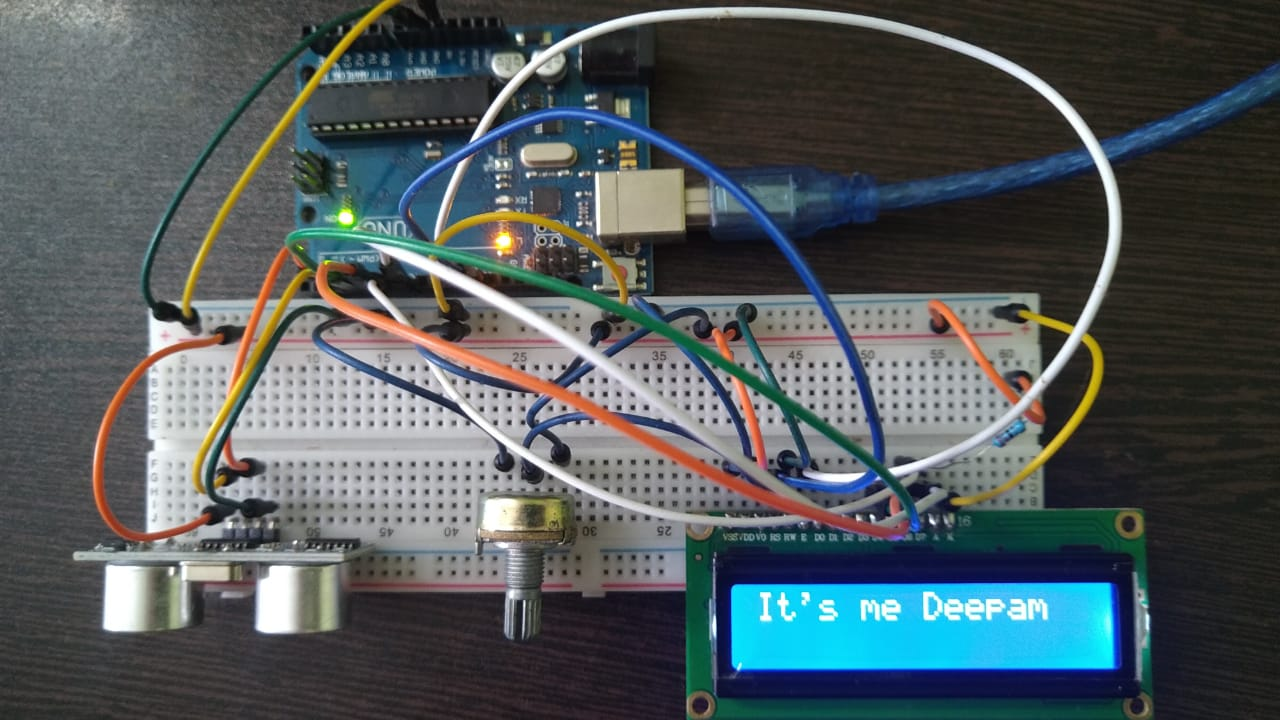
\includegraphics[width=1\textwidth]{lcd_output.jpeg}}
    \caption{LCD screen displaying the output.}
    \label{fig:lcd_output}
\end{figure}

\pagebreak
\subsection{HC-SR04 Ultrasonic sensor interfacing}
\begin{figure}[H]
    \centering
    \fbox{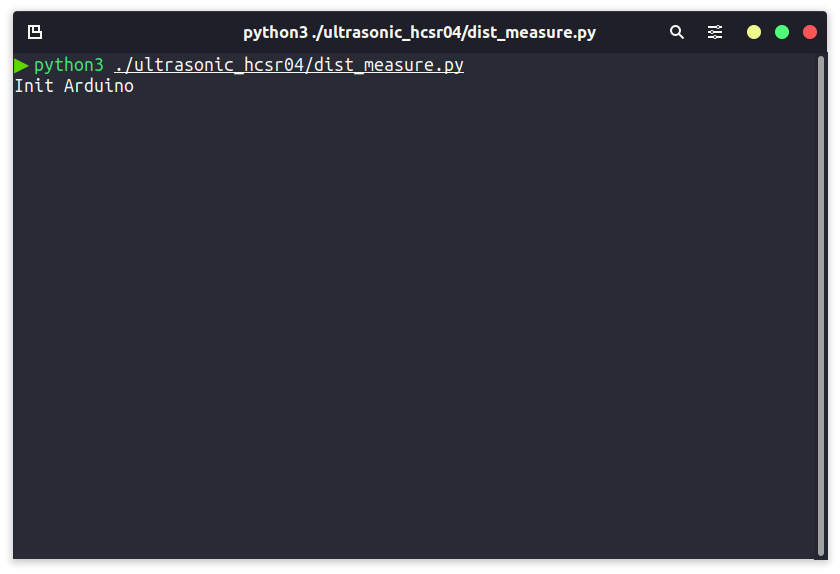
\includegraphics[width=1\textwidth]{us_run.png}}
    \caption{Python console executing Ultrasonic interfacing code}
    \label{fig:us_run}
\end{figure}
\vspace{20pt}
Figure \ref{fig:us_run} shows the execution of the ``dist\_measure.py" python code which initializes the Arduino and the HC-SR04 sensor starts measuring the distance(in cm) and displaying it on the LCD as shown in the Figure \ref{fig:us_output}. The ultrasonic interfacing code makes use of the earlier mentioned LCD module in order to display it on the LCD. In Figure \ref{fig:us_output},a solid object is kept at a distance of 18cm from HC-SR04 sensor on the metric scale. The correct values is also being displayed on the LCD.
\begin{figure}
    \centering
    \fbox{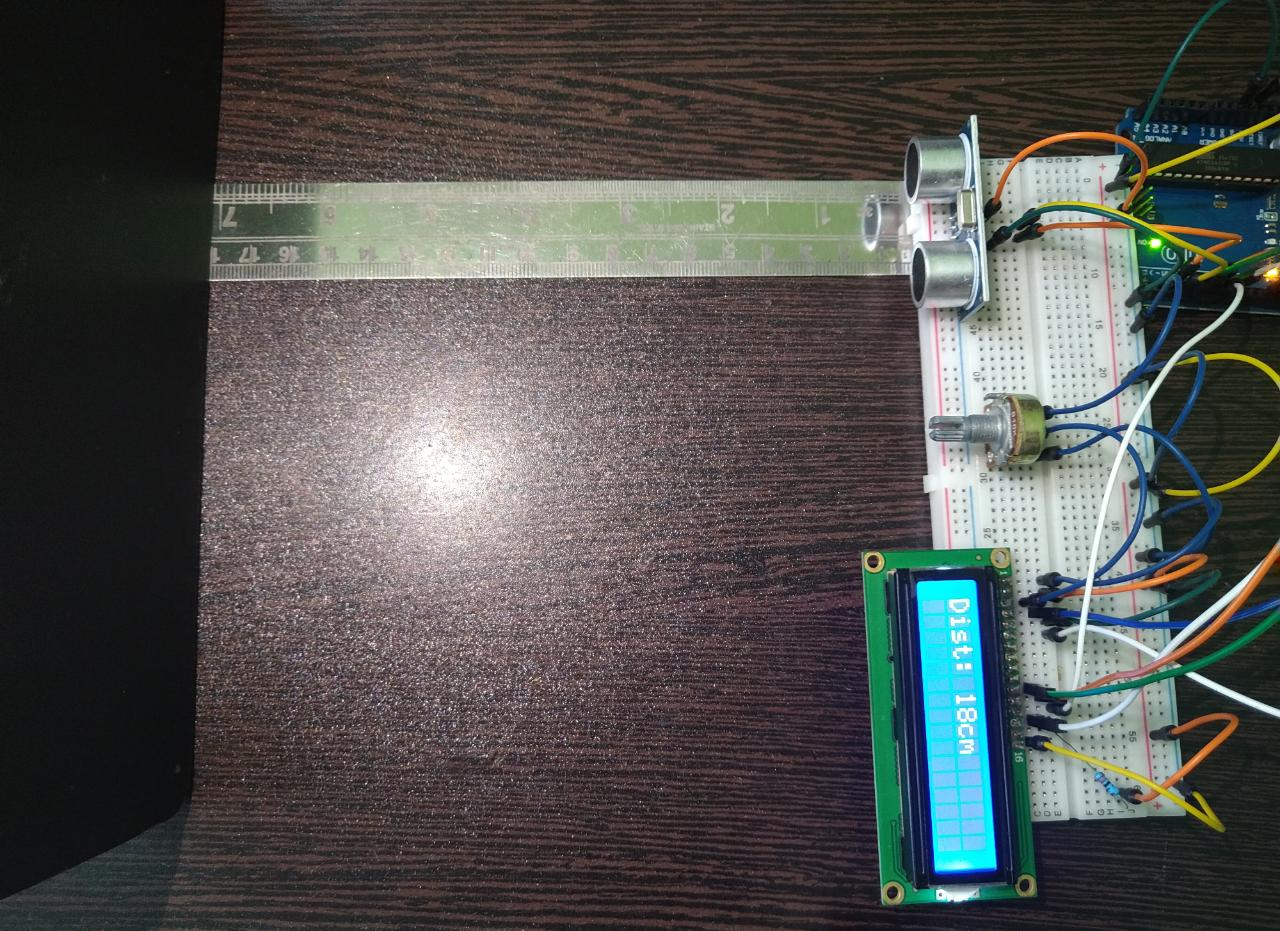
\includegraphics[width=1\textwidth]{us_ouput.jpeg}}
    \caption{Working of HC-SR04 sensor along with 16x2 LCD}
    \label{fig:us_output}
\end{figure}

\end{document}
